\documentclass[conference,10pt]{IEEEtran}
%\documentclass[conference,draft,onecolumn]{IEEEtran}
% useful packages, copy and paste from diff sources

\usepackage[english]{babel}
\usepackage[T1]{fontenc}
\usepackage{cite,url,color} % Citation numbers being automatically sorted and properly "compressed/ranged".
\usepackage{graphics,amsfonts}
\usepackage{epstopdf}
\usepackage[pdftex]{graphicx}
\usepackage[cmex10]{amsmath}
% Also, note that the amsmath package sets \interdisplaylinepenalty to 10000
% thus preventing page breaks from occurring within multiline equations. Use:
\interdisplaylinepenalty=2500
% after loading amsmath to restore such page breaks as IEEEtran.cls normally does.
\usepackage[utf8]{inputenc}
% Useful for displaying quotations
%\usepackage{csquotes}
% Compact lists
%\let\labelindent\relax
\usepackage{enumitem}

%tikz figures
\usepackage{tikz}
\usetikzlibrary{automata,positioning,chains,shapes,arrows}
\usepackage{pgfplots}
\usetikzlibrary{plotmarks}
\newlength\fheight
\newlength\fwidth
\pgfplotsset{compat=newest}
\pgfplotsset{plot coordinates/math parser=false}

\usepackage{array}
% http://www.ctan.org/tex-archive/macros/latex/required/tools/
%\usepackage{mdwmath}
%\usepackage{mdwtab}
%mdwtab.sty	-- A complete ground-up rewrite of LaTeX's `tabular' and  `array' environments.  Has lots of advantages over
%		   the standard version, and over the version in `array.sty'.
% *** SUBFIGURE PACKAGES ***
%\usepackage[tight,footnotesize]{subfigure}
\usepackage{subfig}

\usepackage[top=1.5cm, bottom=2cm, right=1.6cm,left=1.6cm]{geometry}
\usepackage{indentfirst}

\usepackage{times}
% make sections titles smaller to save space
%\usepackage{sectsty}
%\sectionfont{\large}
% enable the use of 'compactitem', a smaller 'itemize'
%\usepackage{paralist}

% MP
% to split equations using dmath env
\usepackage{breqn}
% nice rules in tables
\usepackage{booktabs}

%\setlength\parindent{0pt}
\linespread{1}

% MC
\newcommand{\MC}[1]{\textit{\color{red}MC says: #1}}
\newcommand{\AZ}[1]{\textit{\color{blue}AZ says: #1}}
\newcommand{\MP}[1]{\textit{\color{green}MP says: #1}}

\usepackage{placeins}


%%%%%%%%%%%%%%%%%%%%%%%%%%%%%%%%%%%%%%%%%%
\begin{document}
%%%%%%%%%%%%%%%%%%%%%%%%%%%%%%%%%%%%%%%%%%
\title{Self-Organizing Networks	in LTE: a Q-learning approach to ABS optimization}

\author{\IEEEauthorblockN{Andrea Maracani, Marco Rossanese, Davide Talon}
\IEEEauthorblockA{Department of Information Engineering, University of Padova -- Via Gradenigo, 6/b, 35131 Padova, Italy\\Email: {\tt\{andrea.maracani,marco.rossanese,davide.talon\}@studenti.unipd.it}
}}

\maketitle

\begin{abstract}
In this paper we explain a possible machine-learning approach for the enhanced inter-cell interference coordination (eICIC) in a heterogeneous network (HetNet), where macro and micro cells optimize their downlink transmission in a self-adaptive manner. The idea is to exploit the Q-learning algorithm to guarantee the fair resource sharing between micro and macro cells and so to make the system works in the best performance possible. Indeed this specific reinforcement learning is used to find the optimal policy that leads to the right ABS pattern setting designed specifically for each scenario evaluating only a few parameters and changing dynamically that pattern in order to cope the possible alterations on the environment.\\

\textit{Index  Terms}---SON, Self Optimizing Networks, LTE, eICIC, ABS, reinforcement learning, Q-learning, MONSTeR     
\end{abstract}

%%%%%%%%%%%%%%%%%%%%%%%%%%%%%%%%%%%%%%%%%
\section{Introduction}\label{sec:intro}
%%%%%%%%%%%%%%%%%%%%%%%%%%%%%%%%%%%%%%%%%
The great spreading of mobile devices all over the world represents the fastest adoption of any technology that
our society has ever experienced, faster than the Internet and the earlier generations of mobile
communications. Now tablets, android devices, iPhones, application stores, social media and the data
exchanges between end-users and clouds are all growing at exponential speed. Providing the necessary bandwidth and capacity to the people so they can keep the pace of this growth is a fascinating challenge; then in order to achieve that, a more network densification is required together a full exploitation of the simultaneous presence of micro (coverage radius around 10m-300m) and macro (coverage radius up to 20km) cells, the so called heterogeneous networks (HetNet).\\
The only way these challenges can be cost-effective, efficient and human-handleable is through the use of more automated and autonomous systems, such as Self-Organizing Networks (SON): the goal is to minimize the human intervention in the planning, deployment, optimization and maintenance activities of these new networks.\\
A such SON conceptually must own, as explained by \cite{ramiro2011self}, the following capabilities:
\begin{itemize}
\item Self-Planning: process of identifying the parameter settings of new network elements (like radio parameters of a new eNodeB or a table of neighbor nodes);
\item Self-Deployment: preparation, installation, authentication and delivery of a status report of
a new network node in order to get a "plug and play" approach for each new device;
\item Self-Healing: execution of the routine actions that keep the network operational and/or
prevent problems (this includes the necessary software and hardware upgrades);
\item Self-Optimization is defined as the utilization of measurements and performance indicators
collected by the User Equipments (UEs) and the base stations in order to auto-tune the network
settings.
\end{itemize}
Our work is focused on the last point of the list, more precisely on the improvement of the signal quality and consequently the throughput in a LTE system, trying to minimize the interference between micro and macro cell with an adaptive coordination in downlink transmissions of the antennas (mainly controlling the transmit power patterns).\\
The problem we're facing consists in discovering an optimal trade-off of the radio resources to be assigned between high-power nodes (macro) and low-power nodes (micro). The latter has an higher capacity and consequently an user connected to it will benefit of a better performance, however due to fact that it shares the same frequency band with the macros, low-power nodes are severely affected by the interference from the high-power nodes. In other words, downlink micro transmissions to its UEs could be sorely degraded by high power macro transmission; besides UEs that are close to a micro could end up associating to a macro due to the higher power strength received from the stronger node.\\
So the issue is that, accounting the above scenarios, the micro could be left underutilized and this would turn out to be a bad exploitation of the resources deployed appositely to enhance the connectivity in some areas, with a following decrease of the user performance in comparison with achievable potential capacity.\\
Then with the purpose of promote fair resource sharing, we decided to address the problem trying to stop macros from all the transmissions (some exception signals, like beacons, are always active), for a certain amount of subframes in a frame: this approach is already adopted by LTE and is known as enhanced inter cell interference coordination (eICIC). The period in which macros are "silent" is called Almost Blank Subframe (ABS), period over which micros can transmit with reduced interference.\\
Recalling that a frame is made of ten subframes, the ABS mask, that's the pattern of 0's and 1's where 1 indicates a macro inactive subframe, is found as the result of an optimization problem. The idea is to exploit a reinforcement learning approach, the so called Q-learning technique in order to reach the optimal trade-off of the resources and set the best ABS mask in a self-adaptive manner for each specific scenario.\\
Thanks to the LTE environment simulator MONSTeR, a framework built around the LTE system toolbox available in Matlab, we simulate a great amount of data traffic with the purpose of training the Q-learning: after this period the method involved will yield the best policy for setting the considered mask.
\begin{figure}[h]
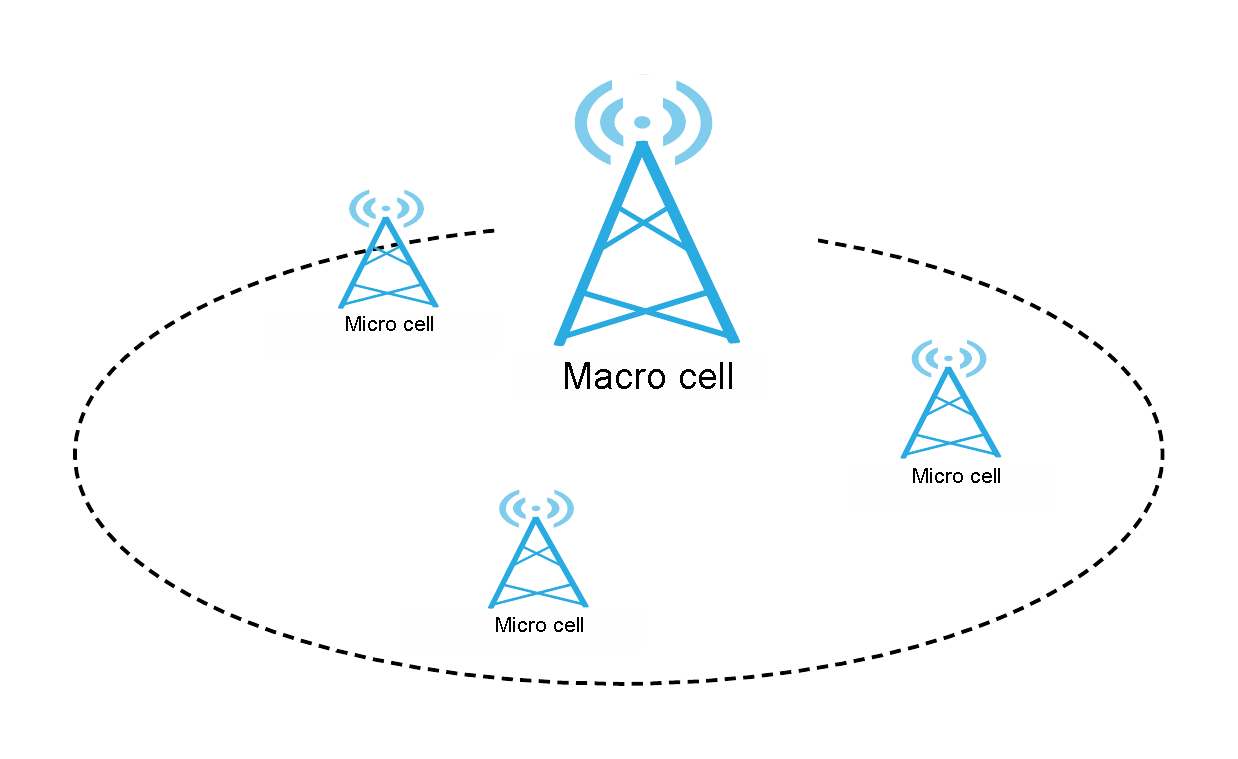
\includegraphics[scale=0.87]{figures/ABS.png}
\caption{Example of a typical HetNet with a macro and some micro used for throughput enhancement in high density utilization area; a micro is placed on the edge of the coverage area for improving the border throughput}
\end{figure}     


\textcolor{red}{\textbf{TO DO (REMEMBER TO ERASE THIS)
\begin{itemize}
\item \textbf{Results: summary of the main findings}
\end{itemize}}}  


%%%%%%%%%%%%%%%%%%%%%%%%%%%%%%%%%%%%%%%%%%%%
\section{Related Work}\label{sec:sota}
%%%%%%%%%%%%%%%%%%%%%%%%%%%%%%%%%%%%%%%%%%%%
In this section we will overview the main proposals in the literature.\\
First of all we must take in account the solution exposed in \cite{simsek2013enhanced} to protect the downlink micro transmissions. Alongside the concept of ABS period they introduced the so called Flexible User Association and Cell selection bias (CSB). As we already know, whenever a UE needs to select a suitable cell for association it chooses the one with the strongest signal and therefore the utilization of the micro mostly of time is neglected.\\
LTE has introduced the bias value $\alpha_i$, that is broadcasted to all the UEs. Hence the UE will choose the right cell maximizing the sum between $\alpha_i$ and the received signal power $P_i$ over each i-th cell in the system; obviously higher bias values are assigned to the micros.\\
The authors of \cite{deb2014algorithms} proposed two algorithms, one for the optimal ABS mask (OPT-ABS) and one for defining the right value for the CBS. The former is split into two parts: the first to search the number of optimal subframes in which the macros are mute and second how to define the optimal ABS pattern. This algorithm turned up to be a NP-hard computational, however they proofed that with a cleaver breakdown of the steps it's implementable and the complexity is scalar with number of cells. Instead the second algorithm compute the biases so that the "association error" (as compared to optimal association) is minimize and this technique shows some shortcomings as the fact is hardly applicable to a non-static scenario and so the beforehand knowledge of the locations is required in order to evaluated which is the best cell in the area.\\
Another noteworthy paper is surely \cite{deb2014algorithms} 

%%%%%%%%%%%%%%%%%%%%%%%%%%%%%%%%%%%%%%
\section{System Model}\label{sec:symo}
%%%%%%%%%%%%%%%%%%%%%%%%%%%%%%%%%%%%%%
The System model is a description of your operating assumptions with related motivation and justification

%%%%%%%%%%%%%%%%%%%%%%%%%%%%%%%%%%%%%%%%%%%%%%%
\section{Results}\label{sec:res}
%%%%%%%%%%%%%%%%%%%%%%%%%%%%%%%%%%%%%%%%%%%%%%%
The Results section contains a selection of the most relevant results with the explanation of their meaning. Please, not that you do NOT have to describe the shape of the curves that can be seen in the figures, but the reasons WHY such curves have that shape!

%%%%%%%%%%%%%%%%%%%%%%%%%%%%%%%%%%%
\section{Conclusions}\label{sec:conclusion}
%%%%%%%%%%%%%%%%%%%%%%%%%%%%%%%%%%%
Conclusions are a superbrief summary of what has been done and highlighting of the "take home message"


\newpage
\nocite{*}
\bibliographystyle{plain}
\bibliography{biblio}
\end{document}
